\documentclass[12pt, a4paper]{article}
\usepackage[utf8]{inputenc}
\usepackage[english,russian]{babel}
\usepackage{amssymb,amsfonts,amsmath,mathtext}
\usepackage{enumerate,indentfirst,tikz,pgf, float}

\topmargin=0mm

\footskip=6mm

\headheight=0pt

\headsep=0pt

\oddsidemargin -0.5cm

\evensidemargin -0.5cm

\textwidth 16.0cm

\textheight 25cm

\topmargin -1.5cm


% ----------- Счетчик задач ------------------------
\newcounter{tasknum}
\newcommand{\task}{\addtocounter{tasknum}{1}
\textbf{Задача \arabic{tasknum}.\,\,}}
%---------------------------------------------------


\begin{document}
\section*{Задания к лекции 1. Базовые понятия теории вероятностей.}

\subsection*{Вариант 1}


\task Из полного набора 28 костей домино наудачу берутся 5 костей.
Найти вероятность того, что среди них будет хотя бы одна кость с шестью очками.

\task Монета подбрасывается 19 раз. Найти вероятность того, чточисло появлений герба четно.

\task В $n$ ящиках размещают $3n$ шаров. Найти вероятность того,
что ни один ящик не пуст.

\task В круг вписан равносторонний треугольник. Точка наудачу бросается в круг. Найти вероятность того, 
что она попадет в треугольник.

\task В урне 7 белых и 3 черных шара. 
Без возвращения извлекаются 3 шара. Известно, что среди них есть черный шар. 
Какова вероятность того, что другие два шара белые?

\task Случайная величина определяется исходом подбрасывания монеты. $0$ -- выпадение <<решки>>,
$1$ -- выпадение <<орла>>. Определить математическое ожидание и дисперсию этой случайной величины, если
исходы не равновероятны: $P$(<<орел>>)$=0.6$, $P$(<<решка>>)$=0.4$.

\task Одна из сторон прямоугольника -- равномерно-распределенная случайная величина на интервале [6, 10]. 
Найти дисперсию площади прямоугольника, если другая его сторона равна 3 cм.

\task Всхожесть семян 36\%. Найти вероятность того, что более 22 семян из 100 прорастут 
(вычислить точное значение с 5-ю десятичными знаками).

\task Вычислить $(0.3, 0.6, 0.8)$-квантили из нормального распределения c параметрами $\mathcal{N}(5, 100)$.

\task Вычислить $(0.3, 0.6, 0.8)$-квантили для равномерного распределения на интервале [5, 15].

\task  Жюри из 5 человек должно быть случайным образом сформировано из 10 мужчин и 5 женщин. 
Найти вероятность того, что жюри будет состоить из двух мужчин и трех женщин. Найти вероятность того, 
что жюри будет состоять только из женщин.


\task На основе некоторого лабораторного эксперимента можно установить взойдет данное семя или нет. Пусть $A$ событие,
состоящее в том, что семя невсхожее; Пусть $B$ событие состоящее в том, что лабораторный тест 
на невсхожесть оказался положительным, т.е. установлено, что семя не взойдет. Известно, что $P(B|A)=0.95$ -- вероятность того, 
что тест определит невсхожесть, если семя невсхожее; $P(B|\overline{A})=0.005$ -- вероятность того, что тест покажет,
что семя невсхожее, хотя на самом деле оно всхожее; 
$P(A)=0.01$ -- вероятность невсхожести (т.е. только приблизительно 1\% от всех семян в популяции не всходят). 
Определить вероятность того, что семя не взойдет, если тест оказался положительным, т.е. найти $P(A|B)?$


\task Даны вероятности отказов работы блоков схемы (Рис.~\ref{block_var1}). Блоки соединены смешанным образом. Вся схема работает, если 
путь в направлении стрелок можно пройти по рабочим блокам. Найти вероятность работы схемы.
\begin{figure}[H]
\centering
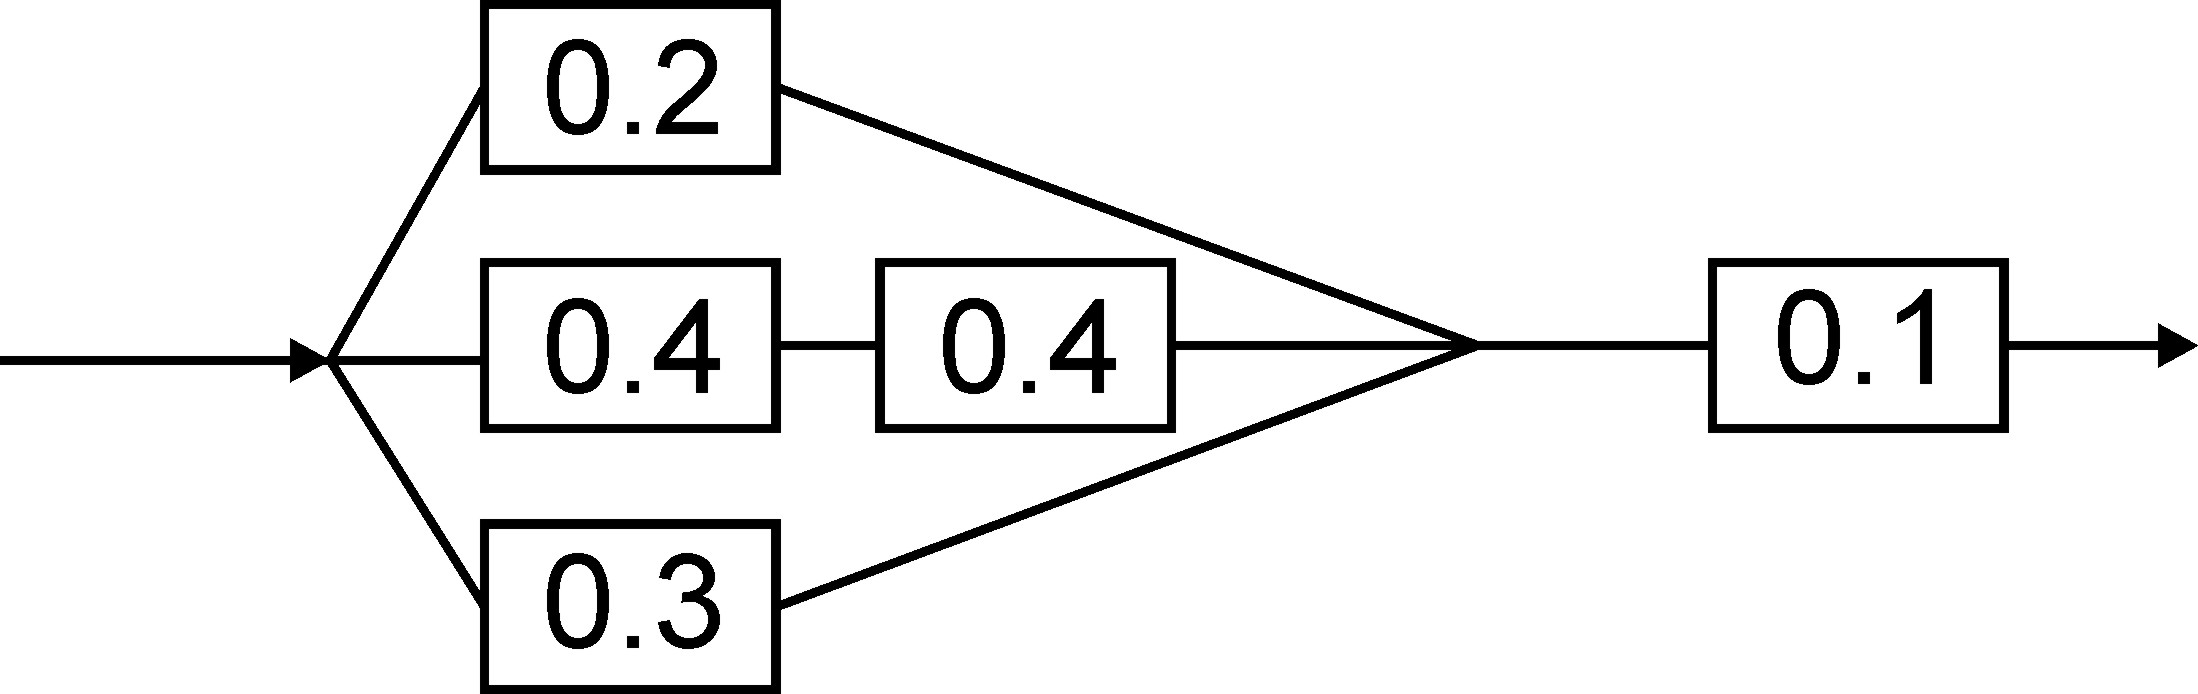
\includegraphics[width=10cm]{schema_var1.jpg}
\caption{Схема соединения блоков.}
\label{block_var1}
\end{figure}

 \task Случайная величина $\xi$ имеет функцию распределения $F_{\xi}(x)$ (Рис.~\ref{cdf_var1}). Найти вероятность $P(\xi>0.5)$.
 \begin{figure}[H]
\centering
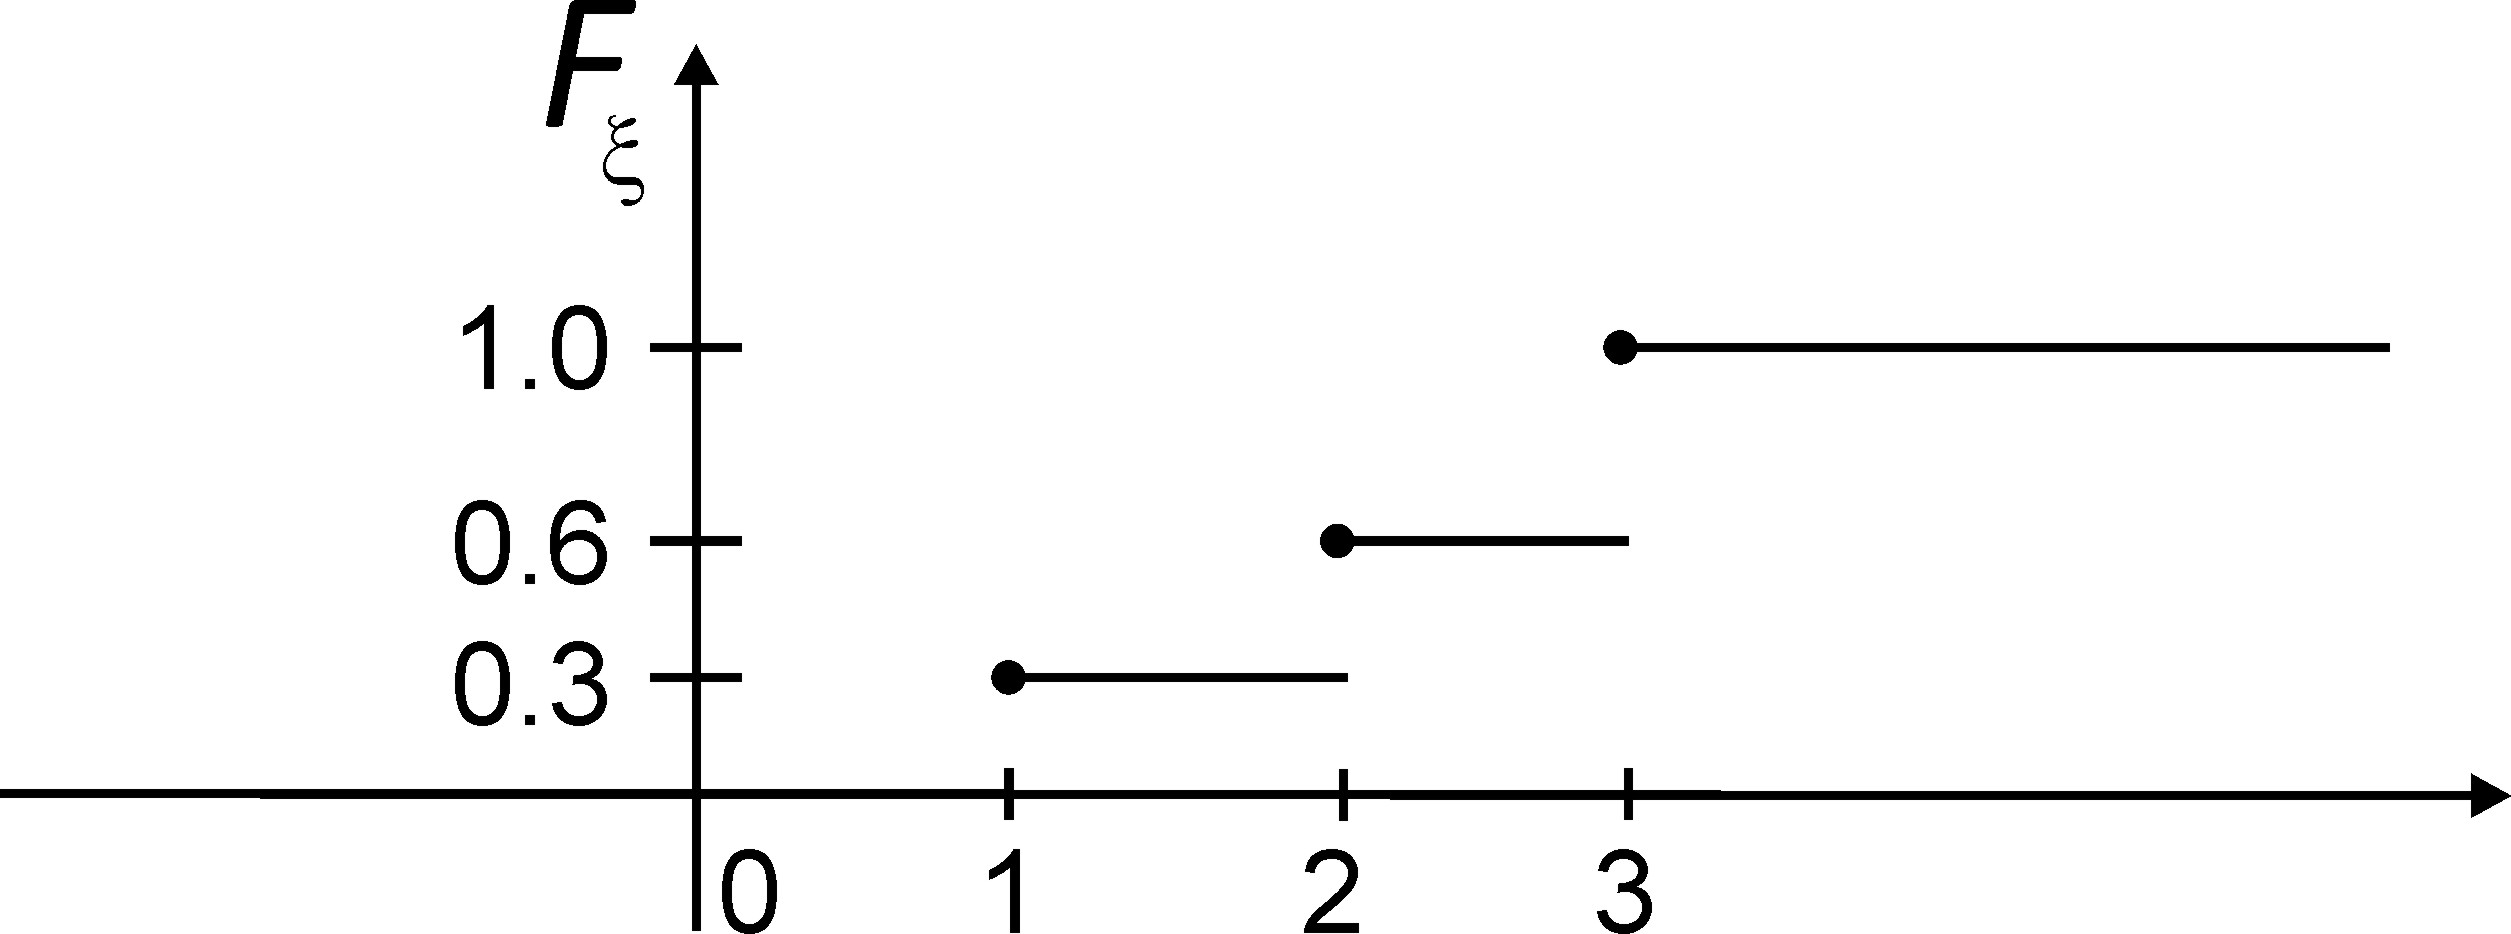
\includegraphics[width=10cm]{cdf1_var1.jpg}
\caption{Функция распределения вероятностей.}
\label{cdf_var1}
\end{figure}


\task Функция плотности распределения случайной величины $\xi$ задана выражением
$$
f_{\xi}=\left\{\begin{array}{l} 1/4, \mbox{при\,} 0<x<1, \\
               3/4, \mbox{при\,} 1<x<2,\\
               0, \mbox{в любом другом случае.} \end{array}\right.
$$
Найти функцию распределения вероятностей $F_{\xi}(x)$.


\clearpage
\newpage
\section*{Задания к лекции 1. Базовые понятия теории вероятностей.}
\subsection*{Вариант 2}
\setcounter{tasknum}{0}
\setcounter{figure}{0}

\task Из полного набора 37 костей домино наудачу берутся 4 кости.
Найти вероятность того, что среди них будет хотя бы одна кость с 2 очками.

\task Монета подбрасывается 15 раз. Найти вероятность того, чточисло появлений герба нечетно.
 
\task В 8 ящиках размещают 16 шаров. Найти вероятность того,
что ни один ящик не пуст.

\task В круг вписан квадрат. Точка наудачу бросается в круг. Найти вероятность того, что она попадет в квадрат.

\task В урне 9 белых и 4 черных шара. 
Без возвращения извлекаются 3 шара. Известно, что среди них есть белый шар. 
Какова вероятность того, что другие два шара белые?

\task Полагая число очков игральной кости (возможные значения от 1 до 6) случайной величиной. 
Найти ее математическое ожидание и дисперсию.
 
\task Одна из сторон прямоугольника -- равномерно-распределенная случайная величина на интервале [10, 15]. 
Найти дисперсию площади прямоугольника, если другая его сторона равна 7 cм.

\task Всхожесть семян 30\%. Найти вероятность того, что более 30 семян из 100 прорастут 
(вычислить точное значение с 5-ю десятичными знаками).

\task Вычислить $(0.1, 0.2, 0.7)$-квантили для нормального распределения c параметрами $\mathcal{N}(5, 100)$. 

\task Вычислить $(0.1, 0.2, 0.7)$-квантили для равномерного распределения на интервале [0, 10]. 

\task Жюри из 5 человек должно быть случайным образом сформировано из 5 мужчин и 10 женщин. 
Найти вероятность того, что жюри будет состоить из двух мужчин и трех женщин. Найти вероятность того, что жюри будет состоять только из женщин.
 
\task На основе некоторого лабораторного эксперимента можно установить взойдет данное семя или нет. Пусть $A$ событие,
состоящее в том, что семя невсхожее; Пусть $B$ событие состоящее в том, что лабораторный тест 
на невсхожесть оказался положительным, т.е. установлено, что семя не взойдет. Известно, что $P(B|A)=0.99$ -- вероятность того, 
что тест определит невсхожесть, если семя невсхожее; $P(B|\overline{A})=0.005$ -- вероятность того, что тест покажет,
что семя невсхожее, хотя на самом деле оно всхожее; 
$P(A)=0.001$ -- вероятность невсхожести (т.е. только приблизительно 0.1\% от всех семян в популяции не всходят). 
Определить вероятность того, что семя не взойдет, если тест оказался положительным, т.е. найти $P(A|B)?$


\task Даны вероятности отказов работы блоков схемы (Рис.~\ref{block_var2}). Блоки соединены смешанным образом. Вся схема работает, если 
путь в направлении стрелок можно пройти по рабочим блокам. Найти вероятность работы схемы.
\begin{figure}[H]
\centering
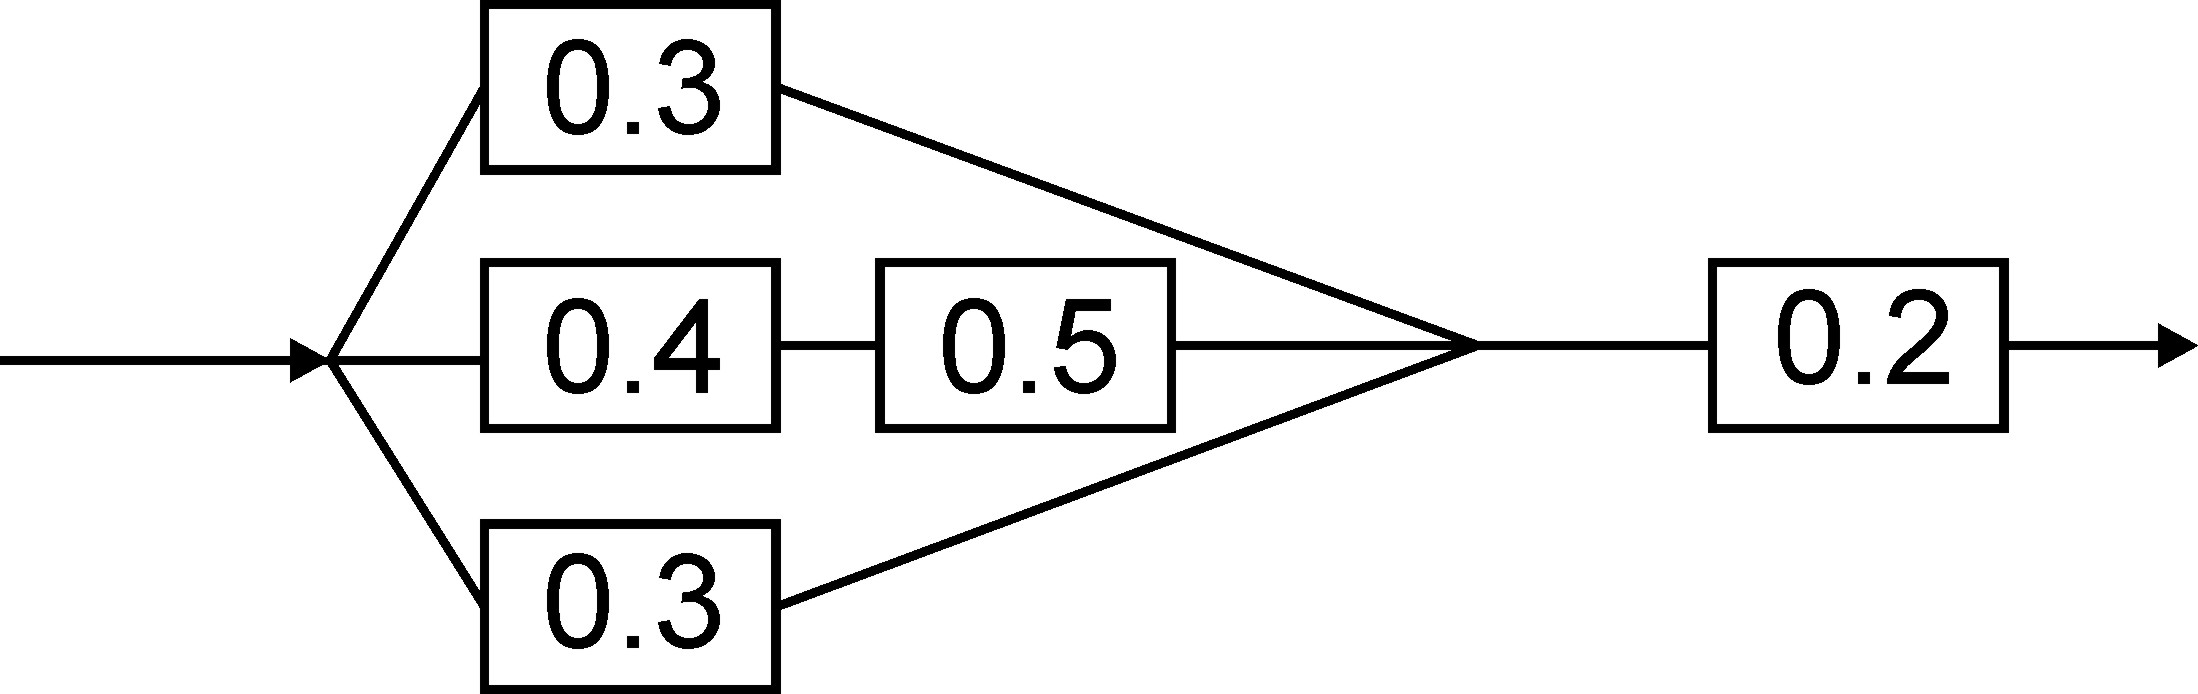
\includegraphics[width=10cm]{schema_var2.jpg}
\caption{Схема соединения блоков.}
\label{block_var2}
\end{figure}


 \task Случайная величина $\xi$ имеет функцию распределения $F_{\xi}(x)$ (Рис.~\ref{cdf_var2}). Найти вероятность $P(\xi>2.5)$.
 \begin{figure}[H]
\centering
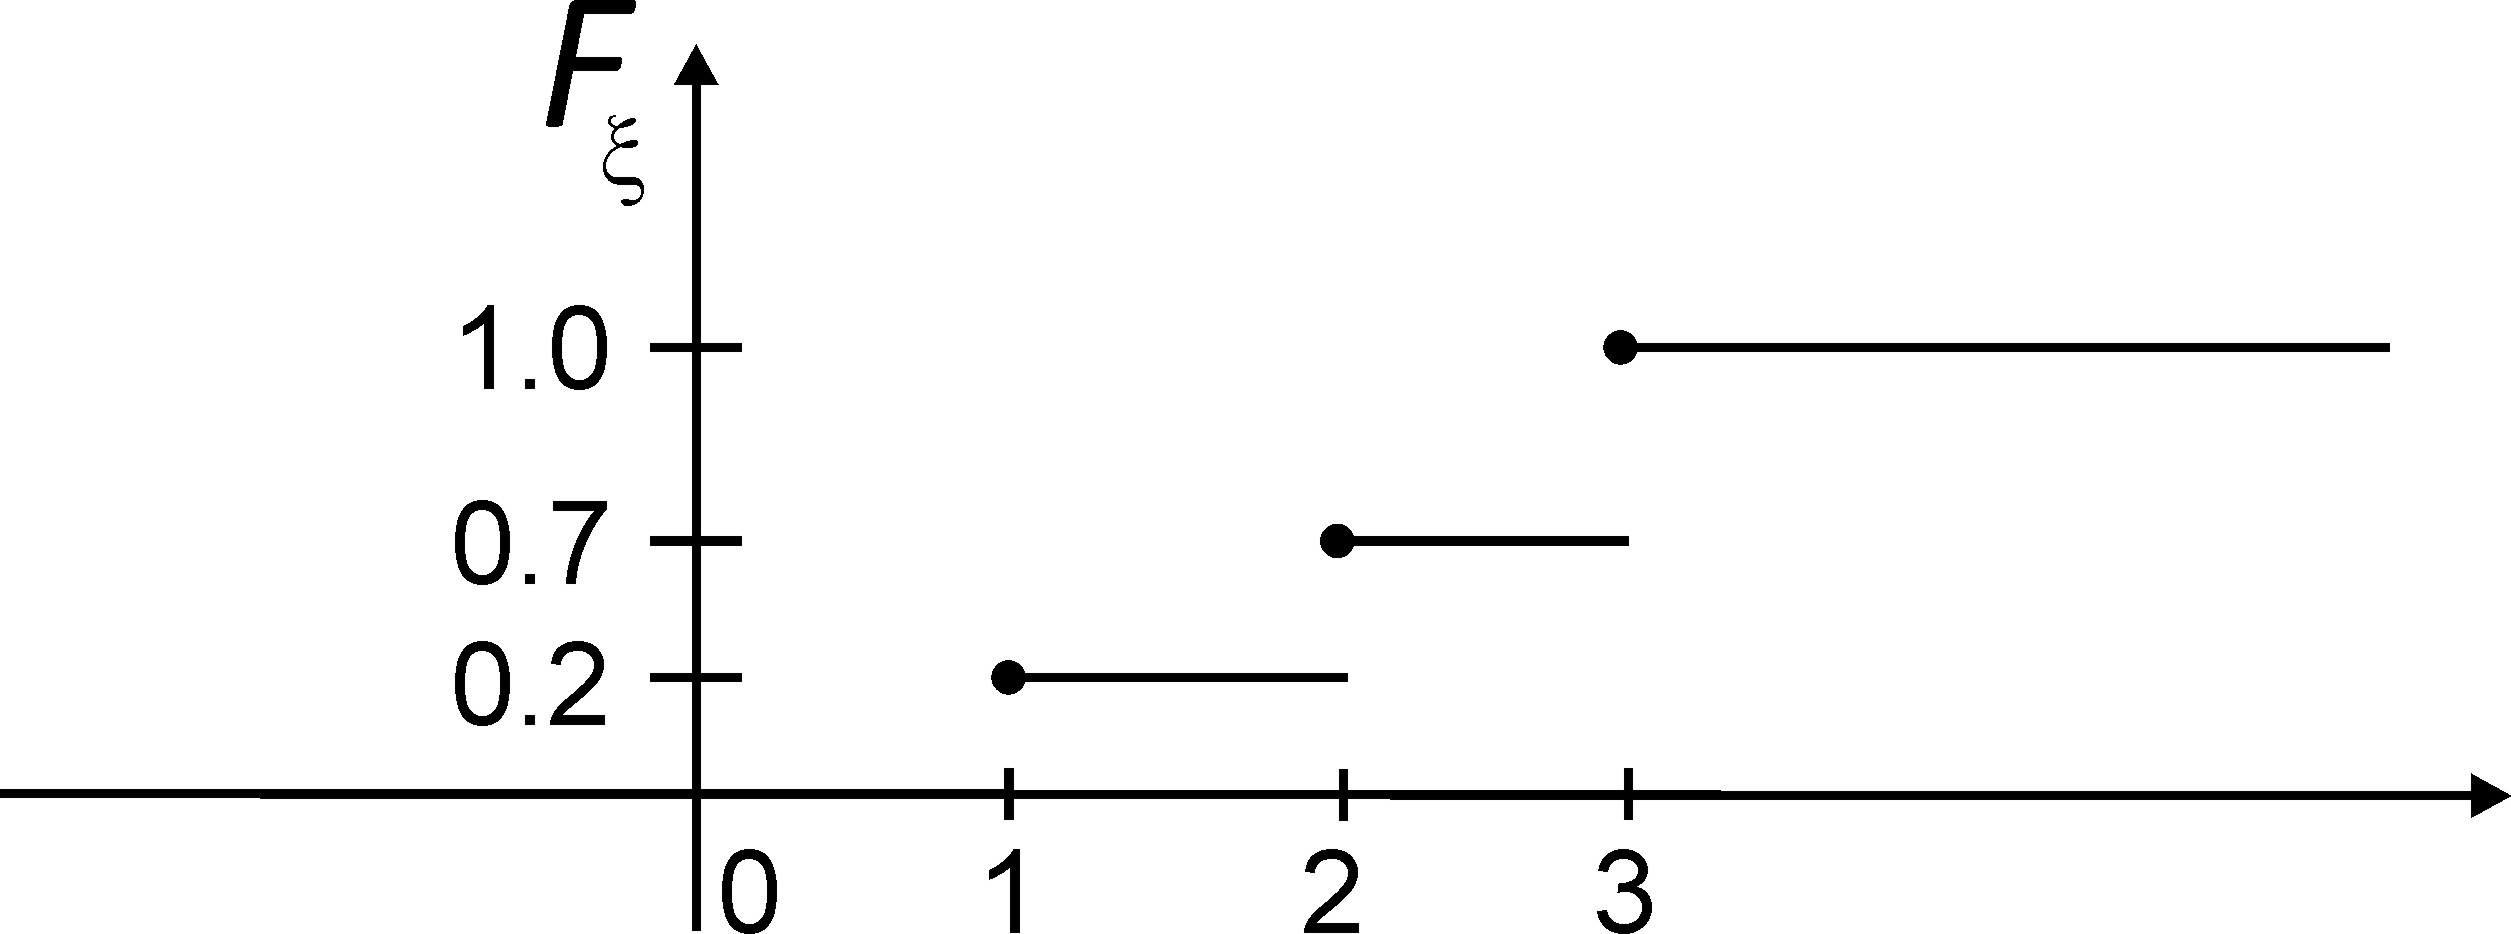
\includegraphics[width=10cm]{cdf1_var2.jpg}
\caption{Функция распределения вероятностей.}
\label{cdf_var2}
\end{figure}
  
 

\task Функция плотности распределения случайной величины $\xi$ задана выражением
$$
f_{\xi}=\left\{\begin{array}{l} 1/3, \mbox{при\,} 0<x<1, \\
               2/3, \mbox{при\,} 1<x<2,\\
               0, \mbox{в любом другом случае.} \end{array}\right.
$$
Найти функцию распределения вероятностей $F_{\xi}(x)$.

 
 
\end{document}



